\documentclass{beamer}

\mode<presentation>
{
\usetheme{Copenhagen}
%\usetheme{Boadilla}
%\usecolortheme{seahorse}
%\useoutertheme{infolines}
%\useoutertheme[compress]{miniframes}
%\setbeamercovered{transparent}
}

%% \mode<presentation>
%% {
%% \usetheme{progressbar}
%% \setbeamercovered{transparent}
%% }

%\usepackage[english]{babel}
\usepackage[english]{babel}
\usepackage[utf8]{inputenc}
\usepackage[T1]{fontenc}

\usepackage{mathptmx}
\usepackage[scaled=.90]{helvet}
\usepackage[T1]{fontenc}
\usepackage{xspace}
%\usepackage{appendixnumberbeamer}
\usepackage[noend]{algorithmic}
%\usepackage[algo2e,vlined,algochapter,ruled,dotocloa]{algorithm2e}
\usepackage{fancybox}
\usepackage{algorithm}
\usepackage[noend]{algorithmic}
\usepackage{amssymb,amsmath}
% \usepackage{ulem}
\usepackage{makecell}
\usepackage{times}
\usepackage{bbding}
\usepackage{color}

\title{An introduction to Machine Learning}
%\subtitle{An introduction to the Data Science workflow\\and an motivation to understand ML}
%\title{The Optimal Swapping Problem during Nuclear Refueling Operations}
\newcommand{\todo}[1]{{\color{red}#1}}

\author{E. Rachelson}

\institute{
\includegraphics[width=1.5cm]{img/isae.jpg}}

\date{}


% This is only inserted into the PDF information catalog. Can be left
% out.
\subject{From Predictive Maintenance to Machine Learning}

\setbeamerfont{bibliography entry author}{shape=\upshape,series=\bfseries,size=\footnotesize}%
\setbeamerfont{bibliography entry title}{shape=\upshape,size=\scriptsize,series=\mdseries}
\setbeamerfont{bibliography entry journal}{shape=\upshape,size=\scriptsize,series=\mdseries}
\setbeamerfont{bibliography entry note}{shape=\upshape,size=\scriptsize,series=\mdseries}

\setbeamercolor{block}{bg=blue,fg=red}

\beamertemplatenavigationsymbolsempty
\setbeamertemplate{footline}[frame number]

\begin{document}

\begin{frame}[plain]
\titlepage
\end{frame}

\begin{frame}{Outline}
\begin{enumerate}
\item General introduction and motivation\\
%{\small \it How does ML fit within your business process.\\
%Why you should take time to understand what's under the hood in ML.}
%\item The importance of data pre-processing\\
%{\small \it A practical illustration.}
\item A geometrical approach to ML
%{\small \it Support Vector Machines and a bit of kernel theory.}
\item A probabilistic approach to ML
%{\small \it Naive Bayes Classification and Gaussian Processes.}
\item From mimicking the human brain to Artificial Neural Networks
\item Deep Learning
%{\small \it Artificial Neural Networks.\\
%Deep Learning.}
\item Commitee-based methods: Decision Trees and Boosting
%{\small \it Decision Trees, Boosting, Bagging and Random Forests.}
%\item Practical session, discussion and conclusion
\item Commitee-based methods: Bagging and Random Forests
\end{enumerate}
\end{frame}

\begin{frame}{Syllabus}
This course offers a discovery of the landscape of Machine Learning through its key algorithms. Although the first session tries to cover the full span of Machine Learning techniques, the subsequent sessions will focus on the Supervized Learning problem and will categorize the algorithms from four distinct points of view (the Bayesian perspective, linear separation, neural networks and ensemble methods). The approach taken mixes voluntarily hands-on practice in Python with theoretical and mathematical understanding of the methods. At the end of the course you will be able to make an informed choice between the main families of ML algorithms depending on the problem at hand, you will have an understanding of the algorithmic and mathematical properties of each family of methods and you will have a basic practical knowledge of the scikit-learn and keras Python libraries.

%% \small
%% By the end of the class, you should be able to:
%% \begin{itemize}
%% \item implement a generic workflow of data analysis for your application field;
%% \item know the main bottlenecks and challenges of data-driven approaches;
%% \item link some field problems to their formal Machine Learning counterparts;
%% \item know the main categories of Machine Learning algorithms and which formal problem they solve;
%% \item know the name and principles of some key methods in Machine Learning:
%% \begin{itemize}
%% \item SVM,
%% \item kernel methods,
%% \item Naive Bayes Classification,
%% \item Gaussian Processes,
%% \item Artificial Neural Networks,
%% \item Deep Learning,
%% \item Random Forests;
%% \end{itemize} 
%% \item know the existence of scikit-learn and its API.
%% \end{itemize}
\end{frame}

\begin{frame}{Course goals}
\small
By the end of the class, you should be able to:
\begin{itemize}
\item implement a generic workflow of data analysis for your application field;
\item know the main bottlenecks and challenges of data-driven approaches;
\item link some field problems to their formal Machine Learning counterparts;
\item know the main categories of Machine Learning algorithms and which formal problem they solve;
\item know the name and principles of some key methods in Machine Learning:
\begin{itemize}
\item SVM and kernel methods,
\item Naive Bayes Classification,
\item Gaussian Processes,
\item Artificial Neural Networks and Deep Learning,
\item Decision Trees,
\item Ensemble methods: Boosting, Bagging, Random Forests;
\end{itemize} 
\item know the basics of scikit-learn and keras.
\end{itemize}
\end{frame}

\begin{frame}{Course material}
\small\url{https://github.com/erachelson/MLclass}
\end{frame}

\begin{frame}{Machine Learning}
\begin{center}
Let's talk about Machine Learning.\\
~\\
Keywords?\\
Applications?\\
Purpose?\\
Algorithms?
\end{center}
%% Let's list and discuss some cases from your experience and from the literature.
%% \begin{itemize}
%% \item ~[Your cases here!]
%% \item Predictive maintenance%(RUL/TTF prediction, proba of failure, anomaly detection)
%% \item Market segmentation%(grouping customer habits)
%% \item Demand forecast
%% \item Preliminary design studies
%% \item Clinical diagnosis
%% \item Documentation management.
%% \item Satellite imaging
%% \end{itemize}
\end{frame}

\begin{frame}{From tasks, to data, to ML}
For all these keywords, let's fill the table below, to build a common understanding of:
\begin{itemize}
\item the nature of data at stake
\item the different tasks to automate
\item the difficulties
\end{itemize}
~\\
~\\
\footnotesize
\begin{tabular}{|c|c|c|c|c|c|}
\hline
\thead{\begin{minipage}{1.3cm}\centering Use case\end{minipage}} & \thead{\begin{minipage}{1.3cm}\centering Type of data\end{minipage}} & \begin{minipage}{1.3cm}\centering Properties of data\end{minipage} & \begin{minipage}{1.3cm}\centering Task to automate\end{minipage} & \begin{minipage}{1.3cm}\centering Difficulties\end{minipage} & \begin{minipage}{1.3cm}\centering Comments\end{minipage}\\
\hline
 & & & & & \\
\hline
 & & & & & \\
\hline
 & & & & & \\
\hline
 & & & & & \\
\hline
\end{tabular}
\end{frame}

\begin{frame}{The Data Scientist perspective}
\centering 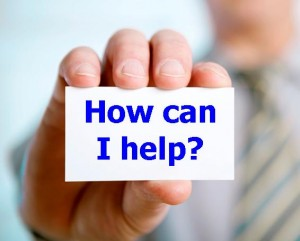
\includegraphics[width=6cm]{img/How-can-i-help.jpg}
\end{frame}

\begin{frame}{Identified needs}
Let's take the example of Predictive Maintenance.\\
~\\
We would like to build automated tools for the following tasks:
\begin{itemize}
\item Visualize system state
\item Identify anomalies
\item Predict Remaining Useful Life (RUL) / Time To Failure (TTF)
\item Predict failure occurrence or probability at a given horizon
\end{itemize}
All this, in order to base our maintenance strategy on the (inferred) system state, rather than a general statistical trend.\\
~\\
\begin{block}{}
Can you relate this task decomposition to the other use-cases we've seen earlier?
\end{block}
Traditionally, all this is based on user expertise.\\
Let's take a data-driven approach.
\end{frame}

\begin{frame}{Data analysis workflow}
\begin{enumerate}
\item<1-> Collect
\item<2-> Analyze
\item<3-> Deploy
\item<4-> Decide
\end{enumerate}
\begin{overlayarea}{10cm}{4cm}
\begin{block}{}
\only<1>{
\begin{itemize}
\item Sensors deployment
\item Historical data collection
\item Integrated storage (datawarehouses) and retrieval issues
\end{itemize}
$\rightarrow$ Extract-Transform-Load (ETL) process\\
More on ETL: \href{https://www.sas.com/en_us/insights/data-management/what-is-etl.html}{[link]}.\\
The \emph{data engineer}'s job: data quality, management, availability.
}
\only<2>{
\begin{itemize}
\item data cleaning
\item feature selection / engineering
\item performance criteria
\item algorithm selection
\item parameters tuning
\end{itemize}
The \emph{data analyst} or \emph{data scientist}'s job.\\
But can't be disconnected from field engineers on the task.
}
\only<3>{
\begin{itemize}
\item Deploy solution in your operational process
\item Make things usable
\end{itemize}
}
\only<4>{
\begin{itemize}
\item Improve your decisions
\end{itemize}
End-user.\\
Job title depends on your professional field.
}
\only<5>{
Need to automate as many steps as possible in this workflow\\
\hspace{2cm}$\rightarrow$ data-driven approaches\\
\hspace{2cm}$\rightarrow$ Machine Learning for step 2
}
\end{block}
\end{overlayarea}
\end{frame}

\begin{frame}{A word on data quality}
\begin{itemize}
\item amount of data: data is often abundant but crucial data is often scarce
\item noise, errors, missing data, outdated data: reliability
\item high-dimensional data
\item class imbalance
\item heterogeneous data (scalars, booleans, time series, images, text, \ldots)
\end{itemize}
All these will influence your algorithmic design or choices.\\
~\\
So let's talk about algorithms to see how we can solve the problems listed earlier.
\end{frame}

\begin{frame}{Machine Learning}
\centering
Machines that learn?\\
Let's try to give a general definition.\\
~\\
\visible<2>{Machine learning is a field of computer science that gives computer systems the ability to ``learn'' (i.e. progressively improve performance on a specific task) with data, without being explicitly programmed.
\begin{flushright}
{\footnotesize (\href{https://en.wikipedia.org/wiki/Machine_learning}{Wikipedia)}}
\end{flushright}}
\end{frame}

\begin{frame}{ML examples}
\begin{overlayarea}{\textwidth}{5cm}
\begin{itemize}
\item<1-> Given 20 years of clinical data, will this patient have a second heart attack in the next 5 years?
\item<2-> What price for this stock, 6 months from now?
\item<3-> Is this handwritten number a 7?
\item<4-> Is this e-mail a spam?
\item<5-> Can I cluster together customers? press articles? genes?
\item<6-> What is the best strategy when playing video games? or poker?
\end{itemize}
\end{overlayarea}
\begin{overlayarea}{\textwidth}{2.5cm}
\begin{center}
\only<1>{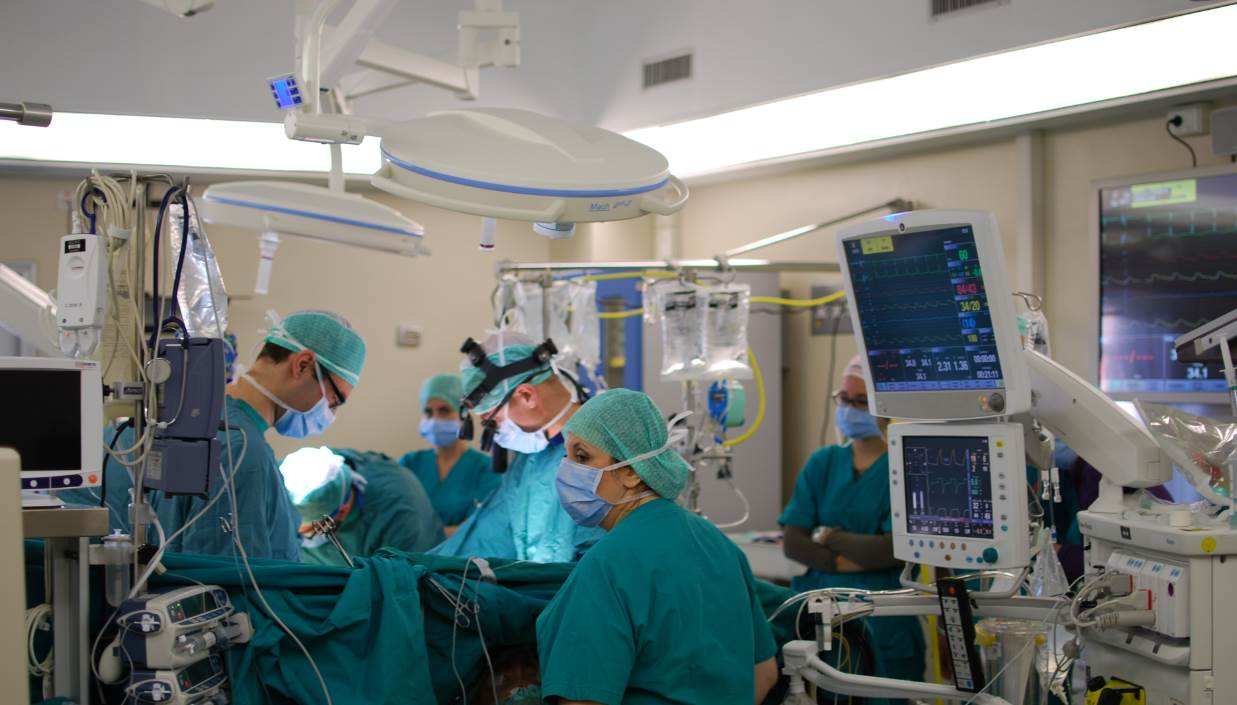
\includegraphics[height=2.5cm]{img/surgery.jpg}}
\only<2>{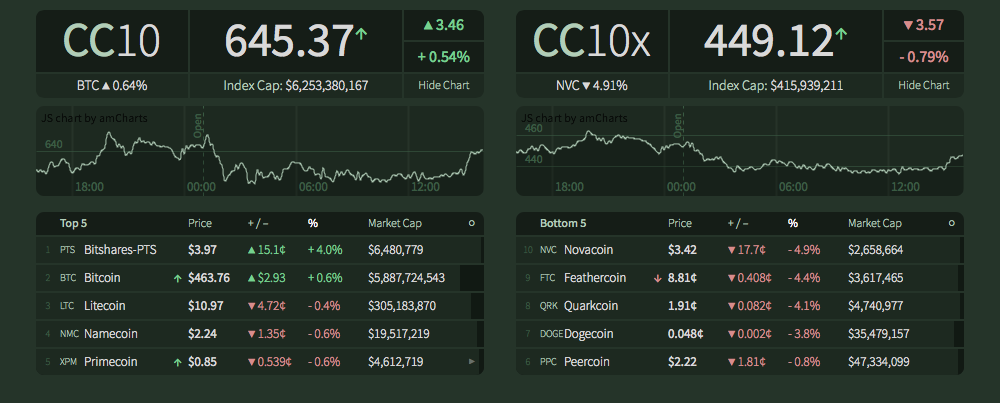
\includegraphics[height=2.5cm]{img/finance.png}}
\only<3>{
\includegraphics[height=2.5cm]{img/seven.jpg}}
\only<4>{\begin{tabular}{rl}
\begin{minipage}{0.9cm}

\includegraphics[height=1cm]{img/message.jpg}
\end{minipage} & \textbf{Enlarge your thesis!}
\end{tabular}}
\only<5>{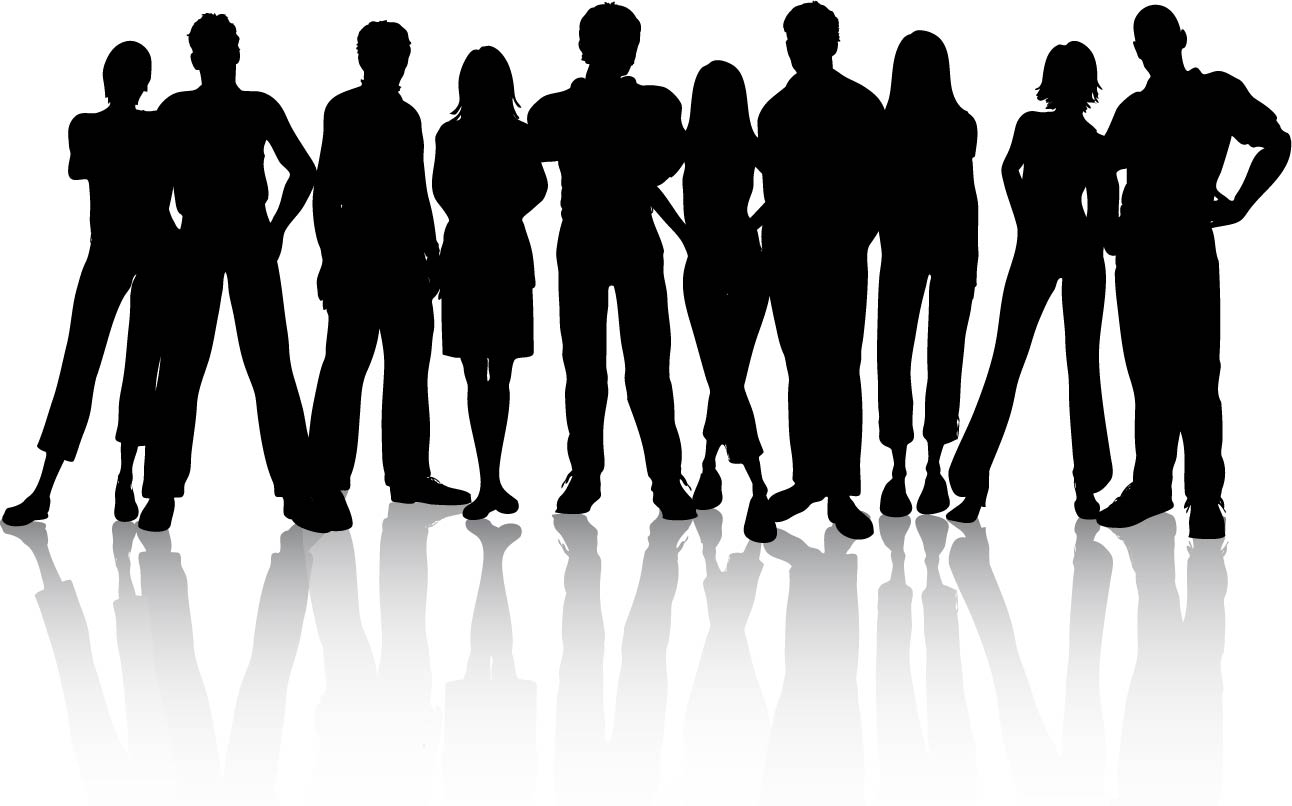
\includegraphics[height=2.5cm]{img/people.jpg}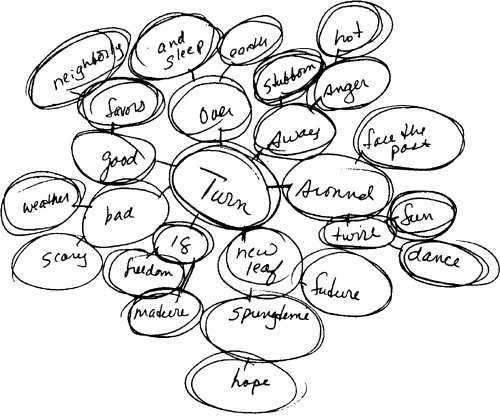
\includegraphics[height=2.5cm]{img/words.jpg}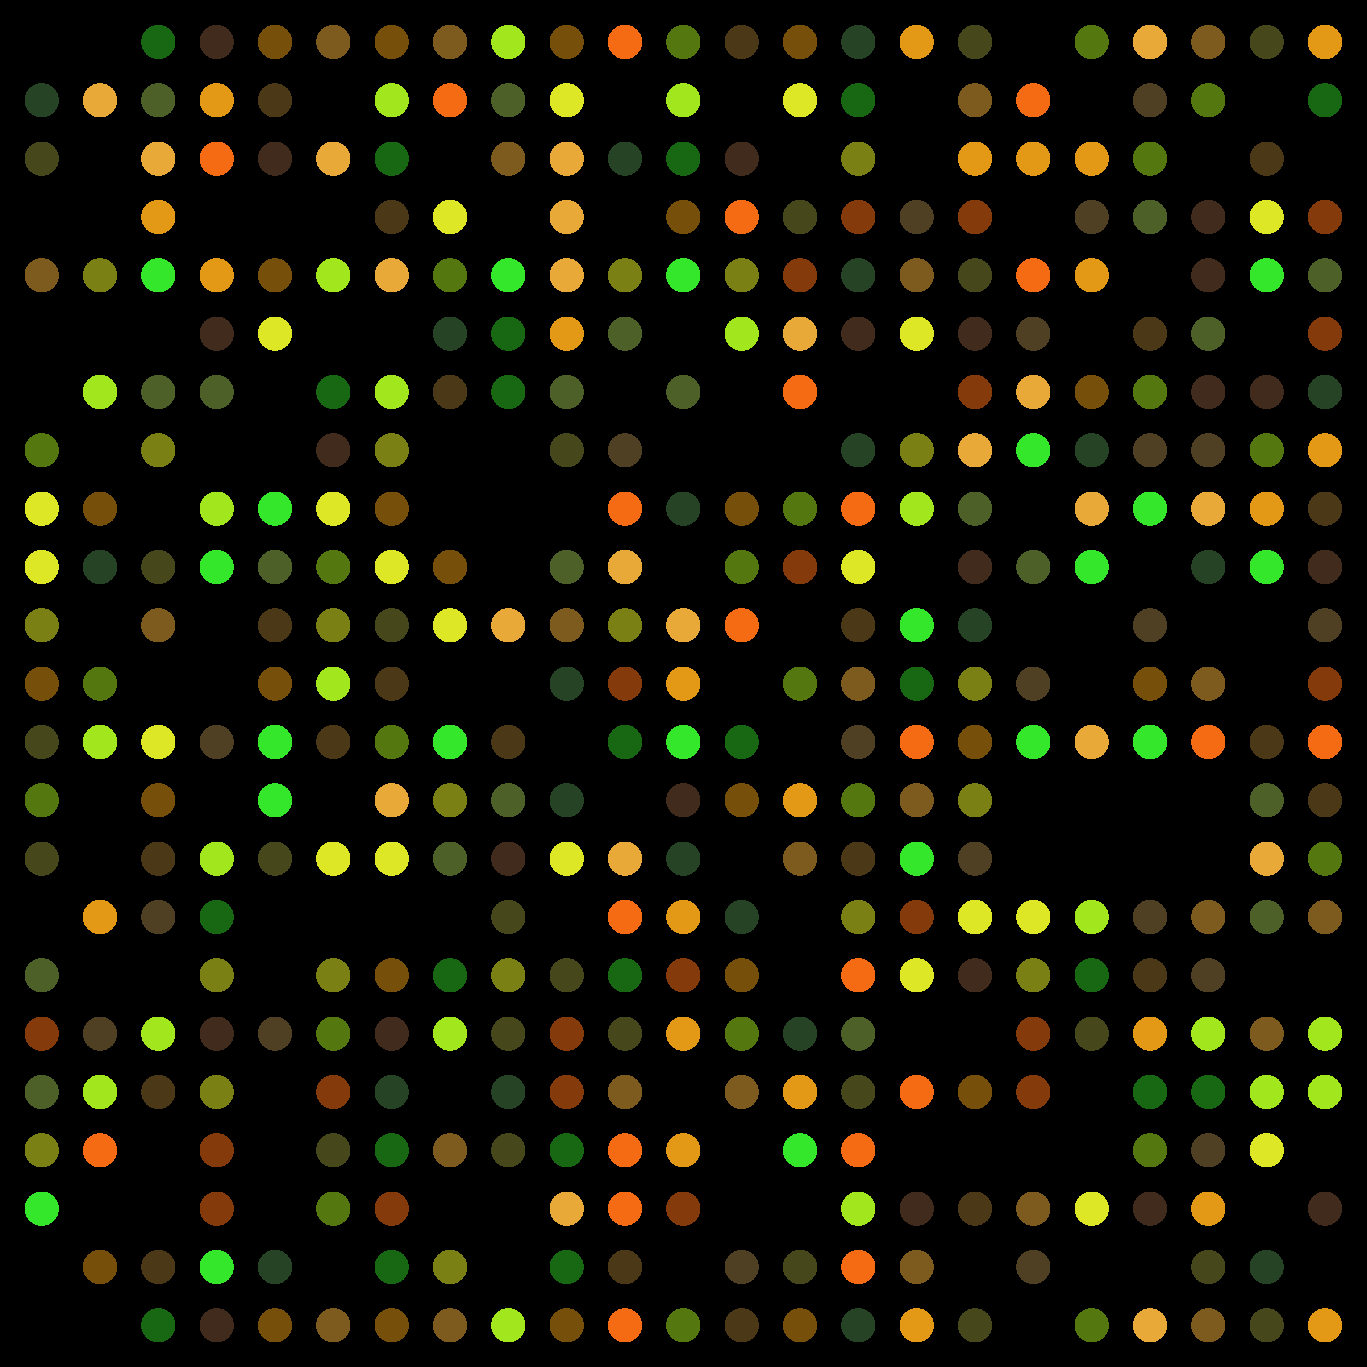
\includegraphics[height=2.5cm]{img/DNA_microarray.pdf}}
\only<6>{
\includegraphics[height=2.5cm]{img/counterstrike2.jpg}~~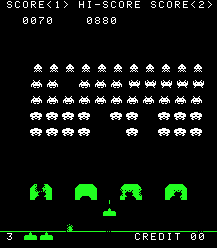
\includegraphics[height=2.5cm]{img/spaceinv.png}~~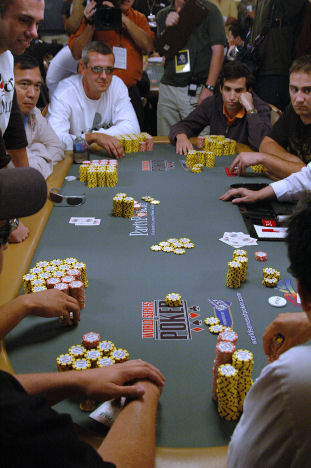
\includegraphics[height=2.5cm]{img/poker2.jpg}}
\end{center}
\end{overlayarea}
\begin{overlayarea}{\textwidth}{1cm}
\tiny Image sources:
\only<1>{\href{https://commons.wikimedia.org/wiki/File:Cardiac_surgery_operating_room.jpg}{Wikimedia commons}}\only<2>{\href{https://commons.wikimedia.org/wiki/File:Crypto_Composite_home_page.png}{Wikimedia commons}}\only<3>{\href{http://www.urbanthreads.com/productImages/regularSize/UTH4670.jpg}{Seven.jpg}}\only<4>{\href{https://www.iconfinder.com/icons/118781/mail_message_new_icon}{Iconfinder}}\only<5>{\href{http://clipart-library.com/white-people-cliparts.html}{People.jpg} / 
\href{http://journals.sagepub.com/doi/pdf/10.1207/s15328023top1701_10}{Writing to Discuss: Use of a Clustering Technique} / 
\href{https://commons.wikimedia.org/wiki/File:DNA_microarray.svg}{DNA microarray}}\only<6>{\href{https://en.wikipedia.org/wiki/File:Counter-Strike_Source_(box_art).jpg}{CS:source} / \href{https://en.wikipedia.org/wiki/File:SpaceInvaders-Gameplay.gif}{Space invaders} /  \href{https://commons.wikimedia.org/wiki/File:2006_WSOP_Main_Event_Table.jpg}{poker}}
\end{overlayarea}
\end{frame}

\begin{frame}{ML tasks}
What does ML do? 3 main tasks.\\
~\\
\begin{tabular}{|c|c|c|c|}
\hline
\makecell[{{p{0.07\textwidth}}}]{\textbf{Task}} &
\makecell[{{p{0.27\textwidth}}}]{\centering \textbf{Supervized\\ Learning}} & \makecell[{{p{0.27\textwidth}}}]{\centering \textbf{Unsupervized Learning}} & \makecell[{{p{0.27\textwidth}}}]{\centering \textbf{Reinforcement Learning}}\\
\hline
\makecell[{{p{0.07\textwidth}}}]{\textbf{Goal}} &
\makecell[{{p{0.27\textwidth}}}]{\centering Learn a function, $f(x)=y$} & \makecell[{{p{0.27\textwidth}}}]{\centering Find groups and correlations, $x\in C$} & \makecell[{{p{0.27\textwidth}}}]{\centering Optimal control, $f(x)=u \ / \ \max\sum r$}\\
\hline
\makecell[{{p{0.07\textwidth}}}]{\textbf{Data}} &
\makecell[{{p{0.27\textwidth}}}]{\centering $\{(x,y)\}$} & \makecell[{{p{0.27\textwidth}}}]{\centering $\{x\}$} & \makecell[{{p{0.27\textwidth}}}]{\centering $\{(x,u,r,x')\}$}\\
\hline
\makecell[{{p{0.07\textwidth}}}]{\textbf{Sub-task}} &
\makecell[{{p{0.27\textwidth}}}]{\centering Classification, Regression} & \makecell[{{p{0.27\textwidth}}}]{\centering Clustering, Density estimation, Dimensionality reduction} & \makecell[{{p{0.27\textwidth}}}]{\centering Value estimation, Policy optimization}\\
\hline
\makecell[{{p{0.07\textwidth}}}]{\textbf{Algo ex.}} &
\makecell[{{p{0.27\textwidth}}}]{\centering Neural Networks, SVM, Random Forests} & \makecell[{{p{0.27\textwidth}}}]{\centering k-means, PCA, HCA} & \makecell[{{p{0.27\textwidth}}}]{\centering Q-learning}\\
\hline
\makecell[{{p{0.07\textwidth}}}]{\textbf{Appli ex.}} &
\makecell[{{p{0.27\textwidth}}}]{\centering Spam filtering, load inference} & \makecell[{{p{0.27\textwidth}}}]{\centering Topic models, dataviz} & \makecell[{{p{0.27\textwidth}}}]{\centering Atari games, robotics}\\
\hline
\end{tabular}
\end{frame}

\begin{frame}{Vocabulary}
\begin{center}
\begin{tabular}{cc}
inputs & outputs\\
independent variables & dependent variables\\
predictors & responses\\
features & targets\\
$X$ (random variables) & $Y$ (random variables)\\
$x_i$ (observation of X) & $y_i$ (observation of Y)
\end{tabular}
\end{center}
\end{frame}

\begin{frame}{Evaluation criteria 1/3}
Evaluating supervized ML methods: what do we really want?\\
~\\
\underline{Ability to fit the training data (regression):}
\begin{itemize}
\item Mean Square Error, \href{https://en.wikipedia.org/wiki/Coefficient_of_determination}{coefficient of determination}.
$$MSE = \frac{1}{N}\sum_i \left(y_i - f(x_i)\right)^2$$
$$R^2 = 1-\frac{\sum_i \left(y_i - f(x_i)\right)^2}{\sum_i \left(y_i - \bar{y}\right)^2}$$
\end{itemize}
\begin{center}
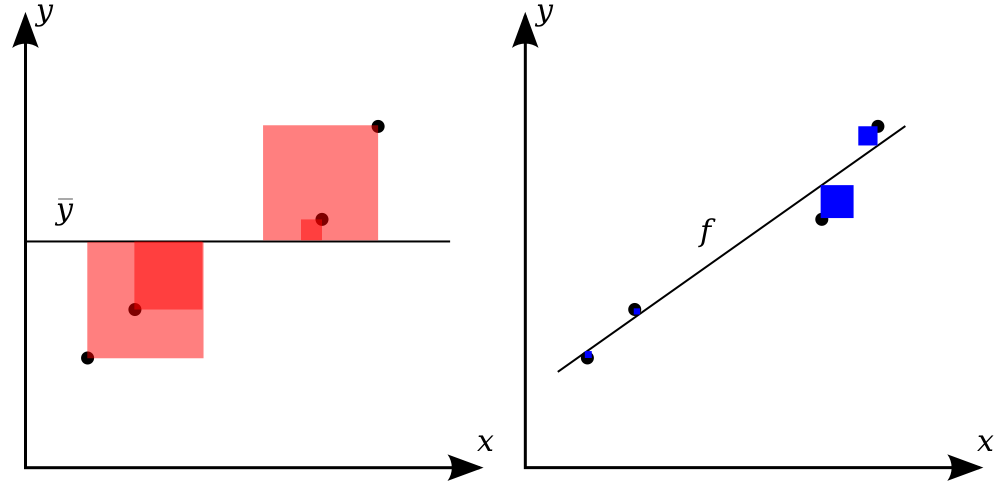
\includegraphics[width=6cm]{img/R2.png}\\
\tiny Image source: \href{https://commons.wikimedia.org/wiki/File:Coefficient_of_Determination.svg}{Wikimedia commons}
\end{center}
\end{frame}

\begin{frame}{Evaluation criteria 2/3}
Evaluating supervized ML methods: what do we really want?\\
~\\
\begin{tabular}{ll}
\begin{minipage}{0.65\textwidth}
\underline{Ability to fit the training data (classification):}
\begin{itemize}
\item Accuracy, TP, FP, confusion matrix
{\href{https://en.wikipedia.org/wiki/Precision_and_recall}{[link]}}
$$Acc = \frac{TP+TN}{TP+FP+TN+FN}$$
\item ROC, AUC, {\href{https://en.wikipedia.org/wiki/Receiver_operating_characteristic}{[link]}}
\end{itemize}
\begin{center}
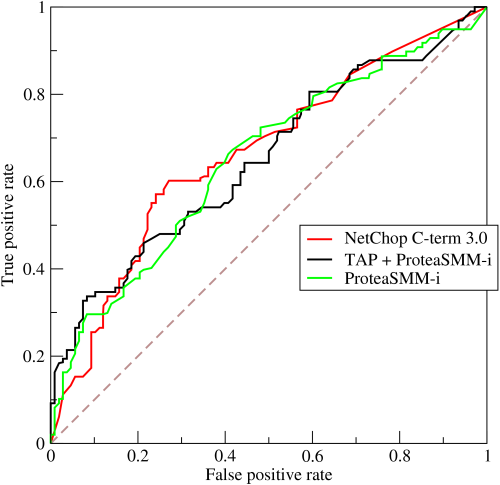
\includegraphics[width=4cm]{img/roc.png}\\
\tiny Image source: \href{https://commons.wikimedia.org/wiki/File:Coefficient_of_Determination.svg}{Wikimedia commons}
\end{center}
\end{minipage} &
\begin{minipage}{0.3\textwidth}
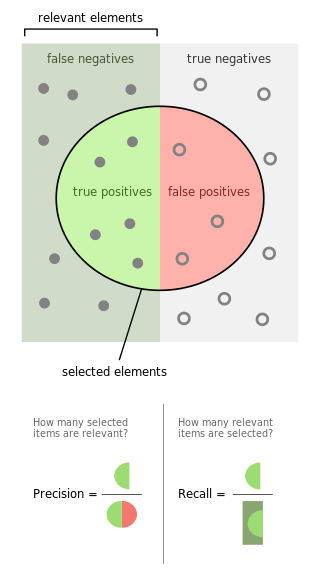
\includegraphics[width=\textwidth]{img/Precisionrecall.png}\\
\tiny Image source: \href{https://commons.wikimedia.org/wiki/File:Roccurves.png}{Wikimedia commons}
\end{minipage}
\end{tabular}
\end{frame}

\begin{frame}{Evaluation criteria 3/3}
Evaluating supervized ML methods: what do we really want?\\
~\\
\underline{Ability to generalize:}
\begin{itemize}
\item Goal: filter out noise, avoid overfitting, generalize to unseen cases.
\item ML Notions:
\begin{itemize}
\item maximize margin
\item minimize difference btw class distributions (cross-entropy \href{https://en.wikipedia.org/wiki/Cross_entropy}{[link]})
\end{itemize}
\end{itemize}
$$H(p,\hat{p}) = \sum_i p(x_i) \log (\hat{p}(x_i)) = \mathbb{E}_p \left(\log(\hat{p})\right)$$
\end{frame}

\begin{frame}{Learning contexts}
Different kinds of learning contexts:\\
\hspace{0.1cm}
\begin{tabular}{lll}
Context & Sample source \\
\hline
{\scriptsize $\blacktriangleright$} Offline, batch, non-interactive & all samples are given at once\\
{\scriptsize $\blacktriangleright$} Online, incremental & samples arrive one after the other\\
{\scriptsize $\blacktriangleright$} Active & the alg. asks for the next sample
\end{tabular}
\end{frame}

\begin{frame}{Misconceptions and clarifications}
\begin{itemize}
\item[AI] ML is only a small (currently fashionable) part of Artificial Intelligence.
\item[BD] Big Data refers to working with datasets that have large Volume, Variety, Velocity (, Veracity, and Value).
\item[DL] Deep Learning is Machine Learning with Deep Neural Networks.
\item[threat] ML / Data Science / Big Data are as much of a threat (to jobs, the society, the economy\ldots) as the combustion engine was in the XIXth century.
\end{itemize}
\end{frame}

\begin{frame}{ML software}
Software:
\begin{itemize}
\item Many free libraries: scikit-learn, tensorflow, caffe\ldots check \url{www.mloss.org} if you're curious.
\item Free environments: Weka, RStudio\ldots
\item Commercial embedded solutions (more or less specialized): Matlab, IBM, Microsoft\ldots
\end{itemize}
\end{frame}

\begin{frame}{Reference textbooks}
\begin{center}
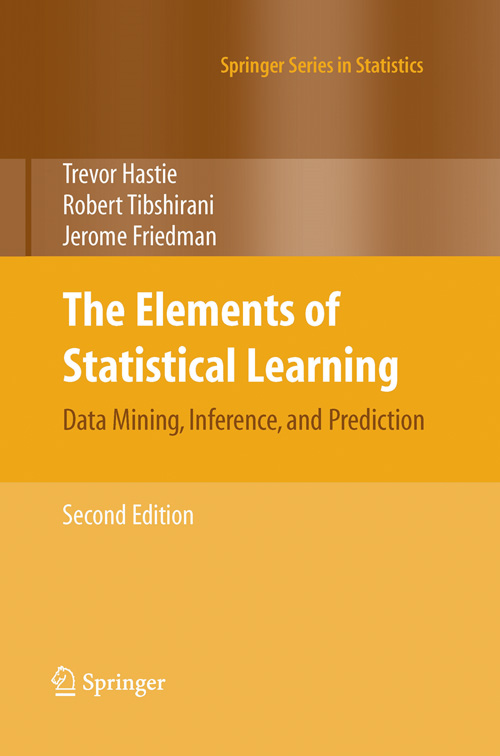
\includegraphics[height=3cm]{img/book.jpg}
\end{center}
\textbf{The Elements of Statistical Learning, second edition.}\\
Trevor Hastie, Robert Tibshirani, Jerome Friedman.\\
\textit{Springer series in Statistics,} 2009.\\
~\\
Other (excellent) references:\\
\textbf{Machine Learning.} T. M. Mitchell.\\
\textbf{Pattern Recognition and Machine Learning.} C. Bishop.\\
\textbf{Deep Learning.} I. Goodfellow, Y. Bengio, A. Courville.\\
\textbf{Hands-on ML with Scikit-Learn and Tensorflow.} A. Géron.
\end{frame}

\begin{frame}{The process of (Un)Supervized Learning}
\begin{center}
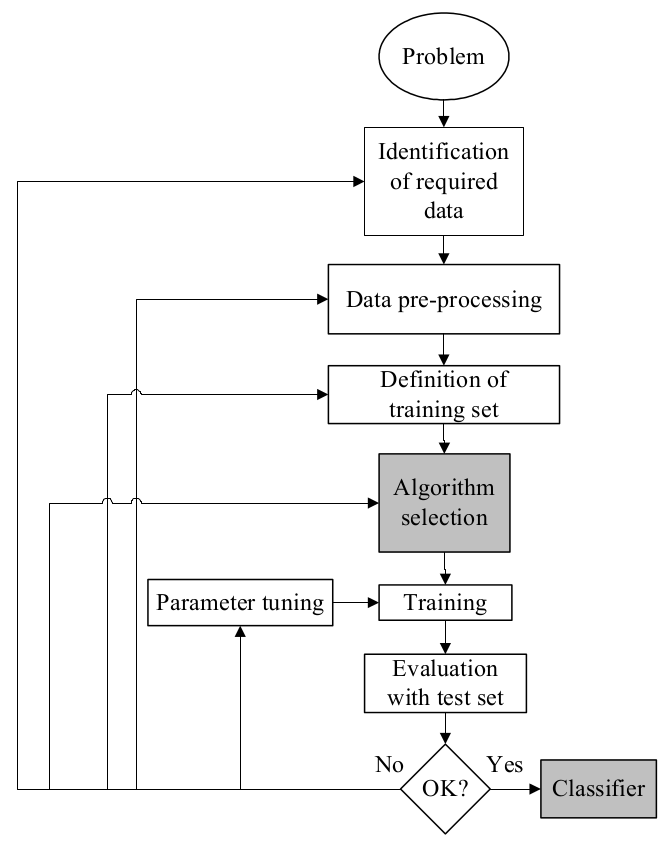
\includegraphics[height=7cm]{img/process.png}
\end{center}
\vspace{-0.5cm}
{\footnotesize From \textbf{Supervized Machine Learning: A Review of Classification Techniques}, S. B. Kotsiantis, \textit{Informatica}, 31:249--268, 2007.}
\end{frame}

\begin{frame}{Relating your needs and ML}
\small
\visible<1->{
Back to the example of Predictive Maintenance tasks.
\begin{itemize}
\item Visualizing system state\\
\hspace{1cm} $\rightarrow$ Dimensionality reduction (Unsupervized learning)
\item Detecting anomalies\\
\hspace{1cm} $\rightarrow$ Density estimation (Unsupervized learning)
\item Predicting RUL or TTF\\
\hspace{1cm} $\rightarrow$ Regression (Supervized learning)
\item Predicting failure in $N$ cycles\\
\hspace{1cm} $\rightarrow$ Classification (Supervized learning)
\end{itemize}
}
\visible<2->{
%~\\
\underline{Thinking like a Maintenance Engineer:}\\
How can I monitor my system to manage my maintenance operations?\\
\underline{Thinking like a Data Scientist:}\\
Is this a supervized or an unsupervized problem? What available data?\\
%~\\
\begin{block}{}
Relate this example to your own field.\\
Now you can start discussing with data scientists to design together the most appropriate method for your data and your problem.
\end{block}
}
\end{frame}

\begin{frame}{A word on scikit-learn}
Scikit-learn = Machine Learning in Python
\begin{itemize}
\item Simple and efficient tools for data mining and data analysis
\item Accessible to everybody, and reusable in various contexts
\item Built on NumPy, SciPy, and matplotlib
\item Open source, commercially usable - BSD license
\item Well documented, with lots of examples
\end{itemize}
\url{http://scikit-learn.org}\\
~\\
Let's take a look at the \href{http://scikit-learn.org/stable/user_guide.html}{documentation's table of contents} to grasp a few more keywords.
\end{frame}

\begin{frame}{Extra things}
\begin{itemize}
\item Installing anaconda, jupyter, etc.
\item ML research: arXiv, JMLR, MLJ, IEEE PAMI, NIPS, ICML, ICLR...
\item datasets: Kaggle, UCI, ImageNet, CIFAR
\item Other algorithms? (scikit-learn documentation or other notebooks)
\item Dataviz: upstream methods (PCA...) and storytelling (Tableau...)
\item What should I look for in a data scientist's CV?
\end{itemize}
\end{frame}

\begin{frame}{Course goals}
\small
By the end of the class, you should be able to:
\begin{itemize}
\item implement a generic workflow of data analysis for your application field;
\item know the main bottlenecks and challenges of data-driven approaches;
\item link some field problems to their formal Machine Learning counterparts;
\item know the main categories of Machine Learning algorithms and which formal problem they solve;
\item know the name and principles of some key methods in Machine Learning:
\begin{itemize}
\item SVM and kernel methods,
\item Naive Bayes Classification,
\item Gaussian Processes,
\item Artificial Neural Networks and Deep Learning,
\item Decision Trees,
\item Ensemble methods: Boosting, Bagging, Random Forests;
\end{itemize} 
\item know the basics of scikit-learn and keras.
\end{itemize}
\end{frame}

\begin{frame}{What you should expect in the remainder of this class}
\begin{itemize}
\item As many intuitive notions as possible,
\item \ldots but also quite a bit of (hopefully painless) math,\\
\item \ldots and a fair amount of hands-on manipulations and demos.
\end{itemize}
\end{frame}

\end{document}
